\documentclass[journal,12pt,twocolumn]{IEEEtran}

\usepackage{setspace}
\usepackage{gensymb}
\singlespacing
\usepackage[cmex10]{amsmath}

\usepackage{amsthm}

\usepackage{mathrsfs}
\usepackage{txfonts}
\usepackage{stfloats}
\usepackage{bm}
\usepackage{cite}
\usepackage{cases}
\usepackage{subfig}

\usepackage{longtable}
\usepackage{multirow}

\usepackage{enumitem}
\usepackage{mathtools}
\usepackage{steinmetz}
\usepackage{tikz}
\usepackage{circuitikz}
\usepackage{verbatim}
\usepackage{tfrupee}
\usepackage[breaklinks=true]{hyperref}
\usepackage{graphicx}
\usepackage{tkz-euclide}

\usetikzlibrary{calc,math}
\usepackage{listings}
    \usepackage{color}                                            %%
    \usepackage{array}                                            %%
    \usepackage{longtable}                                        %%
    \usepackage{calc}                                             %%
    \usepackage{multirow}                                         %%
    \usepackage{hhline}                                           %%
    \usepackage{ifthen}                                           %%
    \usepackage{lscape}     
\usepackage{multicol}
\usepackage{chngcntr}

\DeclareMathOperator*{\Res}{Res}

\renewcommand\thesection{\arabic{section}}
\renewcommand\thesubsection{\thesection.\arabic{subsection}}
\renewcommand\thesubsubsection{\thesubsection.\arabic{subsubsection}}

\renewcommand\thesectiondis{\arabic{section}}
\renewcommand\thesubsectiondis{\thesectiondis.\arabic{subsection}}
\renewcommand\thesubsubsectiondis{\thesubsectiondis.\arabic{subsubsection}}


\hyphenation{op-tical net-works semi-conduc-tor}
\def\inputGnumericTable{}                                 %%

\lstset{
%language=C,
frame=single, 
breaklines=true,
columns=fullflexible
}
\begin{document}

\newcommand{\BEQA}{\begin{eqnarray}}
\newcommand{\EEQA}{\end{eqnarray}}
\newcommand{\define}{\stackrel{\triangle}{=}}
\bibliographystyle{IEEEtran}
\raggedbottom
\setlength{\parindent}{0pt}
\providecommand{\mbf}{\mathbf}
\providecommand{\pr}[1]{\ensuremath{\Pr\left(#1\right)}}
\providecommand{\qfunc}[1]{\ensuremath{Q\left(#1\right)}}
\providecommand{\sbrak}[1]{\ensuremath{{}\left[#1\right]}}
\providecommand{\lsbrak}[1]{\ensuremath{{}\left[#1\right.}}
\providecommand{\rsbrak}[1]{\ensuremath{{}\left.#1\right]}}
\providecommand{\brak}[1]{\ensuremath{\left(#1\right)}}
\providecommand{\lbrak}[1]{\ensuremath{\left(#1\right.}}
\providecommand{\rbrak}[1]{\ensuremath{\left.#1\right)}}
\providecommand{\cbrak}[1]{\ensuremath{\left\{#1\right\}}}
\providecommand{\lcbrak}[1]{\ensuremath{\left\{#1\right.}}
\providecommand{\rcbrak}[1]{\ensuremath{\left.#1\right\}}}
\theoremstyle{remark}
\newtheorem{rem}{Remark}
\newcommand{\sgn}{\mathop{\mathrm{sgn}}}
\providecommand{\abs}[1]{\vert#1\vert}
\providecommand{\res}[1]{\Res\displaylimits_{#1}} 
\providecommand{\norm}[1]{\lVert#1\rVert}
%\providecommand{\norm}[1]{\lVert#1\rVert}
\providecommand{\mtx}[1]{\mathbf{#1}}
\providecommand{\mean}[1]{E[ #1 ]}
\providecommand{\fourier}{\overset{\mathcal{F}}{ \rightleftharpoons}}
%\providecommand{\hilbert}{\overset{\mathcal{H}}{ \rightleftharpoons}}
\providecommand{\system}{\overset{\mathcal{H}}{ \longleftrightarrow}}
	%\newcommand{\solution}[2]{\textbf{Solution:}{#1}}
\newcommand{\solution}{\noindent \textbf{Solution: }}
\newcommand{\cosec}{\,\text{cosec}\,}
\providecommand{\dec}[2]{\ensuremath{\overset{#1}{\underset{#2}{\gtrless}}}}
\newcommand{\myvec}[1]{\ensuremath{\begin{pmatrix}#1\end{pmatrix}}}
\newcommand{\mydet}[1]{\ensuremath{\begin{vmatrix}#1\end{vmatrix}}}
\numberwithin{equation}{subsection}
\makeatletter
\@addtoreset{figure}{problem}
\makeatother
\let\StandardTheFigure\thefigure
\let\vec\mathbf
\renewcommand{\thefigure}{\theproblem}
\def\putbox#1#2#3{\makebox[0in][l]{\makebox[#1][l]{}\raisebox{\baselineskip}[0in][0in]{\raisebox{#2}[0in][0in]{#3}}}}
     \def\rightbox#1{\makebox[0in][r]{#1}}
     \def\centbox#1{\makebox[0in]{#1}}
     \def\topbox#1{\raisebox{-\baselineskip}[0in][0in]{#1}}
     \def\midbox#1{\raisebox{-0.5\baselineskip}[0in][0in]{#1}}
\vspace{3cm}
\title{AI1103-Assignment 3}
\author{Name : Ayush Jha \\ Roll Number: CS20BTECH11006}
\maketitle
\newpage
\bigskip
\renewcommand{\thefigure}{\theenumi}
\renewcommand{\thetable}{\theenumi}
Download all python codes from 
\begin{lstlisting}
https://github.com/ayushjha2612/AI11003/tree/main/Assignment3/Codes
\end{lstlisting}
%
and latex-tikz codes from 
%
\begin{lstlisting}
https://github.com/ayushjha2612/AI11003/tree/main/Assignment3
\end{lstlisting}
\section{GATE Problem 34}
Let X and Y be two statistically independent random variables uniformly distributed in the range (-1, 1) and (-2, 1) respectively. Let $Z = X +Y$ , then the probability that $[Z \leq -2]$ is \\
(A) zero         \hfill  (B) $\dfrac{1}{6}$  \hfill
(C)$\dfrac{1}{3}$      \hfill       (D)$\dfrac{1}{12}$  
\section{Answer}
Option (D) $\dfrac{1}{12}$
\section{Solution}
X and Y are two independent random variables. \\
Let
\begin{align}
    p_X\brak{x} &= \Pr\brak{X=x} \\
    p_Y\brak{y} &= \Pr\brak{Y=y}  \\
    p_Z\brak{z} &= \Pr\brak{Z=z}
\end{align}
be the probability densities of random variables X ,Y and Z. \\
X lies in range(-1,1), therefore,
\begin{align}
    \int_{-1}^{1} p_X\brak{x} \,dx  &=1 \\
    2 \times p_X\brak{x}  &= 1 \\
     p_X\brak{x} =1 /2
\end{align}
Similarly for Y we have,
\begin{align}
    \int_{-2}^{1} p_Y\brak{y} \,dy  &=1 \\
    3 \times p_Y\brak{y}  &= 1  \\
     p_Y\brak{y} =1 /3
\end{align}
The density for X is \\
\begin{align}
\label{eq:_pdf_x}
p_{X}(x)  = 
\begin{cases}
\frac{1}{2} & -1 \le x \le 1
\\
0 & otherwise
\end{cases}
\end{align}
We have ,
\begin{equation}
    Z= X+Y \iff z= x+ y \iff x = z-y
\end{equation}
The density of X can also be represented as,
\begin{align}
\label{eq:pdf_x}
p_{X}(z-y)  = 
\begin{cases}
\frac{1}{2} & -1 \le z-y \le 1
\\
0 & otherwise
\end{cases}
\end{align}
and the density of Y is,
\begin{align}
\label{eq:pdf_y}
p_{Y}(y)  = 
\begin{cases}
\frac{1}{3} & -2 \le y \le 1
\\
0 & otherwise
\end{cases}
\end{align}
The density of Z i.e. $Z= X + Y $ is given by the convolution of the densities of X and Y
\begin{equation}
    p_Z(z) =  \int_{- \infty}^{\infty} p_X(z-y)p_Y(y) \,dy 
\end{equation}
From \ref{eq:pdf_x} and \ref{eq:pdf_y} we have, \\
The integrand is $\dfrac{1}{6}$ when,
\begin{align}
    2 \le y \le 1 \\
    -1 \le z-y \le 1 \\
    z-1 \le y \le z+1
\end{align}
and zero, otherwise. \\
Now when $-3 \le z \le -2$ them we have, 
\begin{align}
    p_Z(z) &=   \int_{-2}^{z+1} \dfrac{1}{6} \,dy  \\
          &= \dfrac{1}{6} \times ( z+1 - (-2)) \\
          &= \dfrac{1}{6}(z+3)
\end{align}
For $ -2 < z \le -1 $,
\begin{align}
    p_Z(z) &=   \int_{-2}^{z+1} \dfrac{1}{6} \,dy  \\
          &= \dfrac{1}{6} \times ( z+1 - (-2)) \\
          &= \dfrac{1}{6}(z+3)
\end{align}
For $ -1 < z \le 0 $,
\begin{align}
    p_Z(z) &=   \int_{z-1}^{z+1} \dfrac{1}{6} \,dy  \\
          &= \dfrac{1}{6} \times ( z+1 - (z-1)) \\
          &= \dfrac{1}{3}
\end{align}
For $ 0 < z \le 2$,
\begin{align}
    p_Z(z) &=   \int_{z-1}^{1} \dfrac{1}{6} \,dy  \\
          &= \dfrac{1}{6} \times ( 1- (z-1)) \\
          &= \dfrac{1}{6}(2-z)
\end{align}
Therefore the density of Z is given by
\begin{align}
\label{eq:pdf_z}
p_{Z}(z)  = 
\begin{cases}
\frac{1}{6}(z+3) & -3 \le z \le -2
\\
\frac{1}{6}(z+3) & -2 < z \le -1
\\
\frac{1}{3} & -1 < z \le 0
\\
\frac{1}{6}(2-z) & 0 < z \le 2
\\
0 & otherwise
\end{cases}
\end{align}
The CDF of Z is defined as,
\begin{equation}
    F_Z(z) = \Pr\brak{Z \le z}
\end{equation}
Now for $ z \le -1 $,
\begin{align}
    \Pr\brak{Z\le z} &=  \int_{-\infty}^{z}p_{Z}(z) \,dz  \\
          &=  \int_{-3}^{z} \dfrac{1}{6}(z+3) \,dz  \\
          &= \dfrac{1}{6} \left(\dfrac{z^2}{2}+3z \right) \Biggr|_{-3}^{z}  \\
          &=  \dfrac{1}{6} \times \left(\left(\dfrac{z^2}{2}+3z \right) - \left(\dfrac{9}{2} -9 \right)\right) \\
          &= \dfrac{z^2+6z + 9}{12} 
\end{align}
Similarly for $z \le 0$,
\begin{align}
    \Pr\brak{Z\le z} &=  \int_{-\infty}^{z}p_{Z}(z) \,dz  \\
          &=  \dfrac{1}{3} + \int_{-1}^{z} \dfrac{1}{3} \,dz  \\
          &= \dfrac{z+2}{3} 
\end{align}
finally for $z \le 2$,
\begin{align}
    \Pr\brak{Z\le z} &=  \int_{-\infty}^{z}p_{Z}(z) \,dz  \\
          &= \dfrac{2}{3} + \int_{0}^{z} \dfrac{1}{6}(2-z) \,dz  \\
         & =  \dfrac{2}{3} +\dfrac{4z- z^2}{12} \\
         & = \dfrac{8 +4z -z^2}{12} 
\end{align}
The CDF is as below, 
\begin{align}
\label{eq:cdf_z}
F_{Z}(z)  = 
\begin{cases}
0 & z < 3
\\
\frac{z^2+6z + 9}{12} &  z \le -1
\\
\frac{z+2}{3} &  z \le 0
\\
\frac{8 +4z -z^2}{12} & z \le 2
\\
1 & z > 2
\end{cases}
\end{align}
So 
\begin{align}
    \Pr\brak{ Z \leq -2} &= F_{Z}(2) \\
                  = \dfrac{1}{12}
\end{align}
i.e. option (D). \\
The plot for PDF of $Z $ can be observed at figure \ref{fig:The PDF of Z} and the plot for CDF of Z is at figure \ref{fig:The CDF of Z}.
\begin{figure}[!ht]
       \centering
    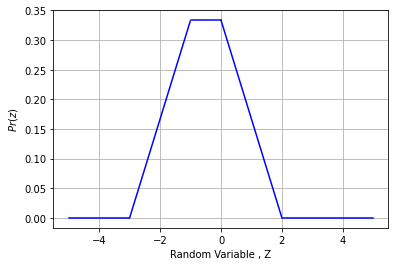
\includegraphics[width=.9\columnwidth] {Assignment_3_PDF.png}
    \caption{The PDF of Z}
    \label{fig:The PDF of Z}
\end{figure}

\begin{figure}[!ht]
       \centering
    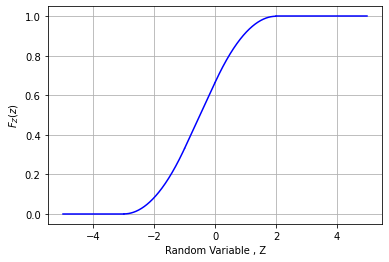
\includegraphics[width=.9\columnwidth] {Assignment_3_CDF.png}
    \caption{The CDF of Z}
    \label{fig:The CDF of Z}
\end{figure}

\end{document}